\documentclass[relatorio]{unemat-comp}
% Opções da classe inf-ufg (ao usar mais de uma, separe por vírgulas)
%   [tese]         -> Tese de doutorado.
%   [dissertacao]  -> Dissertação de mestrado (padrão).
%   [monografia]   -> Monografia de especialização.
%   [relatorio]    -> Relatório final de graduação.
%   [abnt]         -> Usa o estilo "abnt-alf" de citação bibliográfica.
%   [nocolorlinks] -> Os links de navegação no texto ficam na cor preta.
%                     Use esta opção para gerar o arquivo para impressão
%                     da versão final do seu texto!!!

% This package is useful for adding todo notes to the side of the text.
% Use 'disable' option to remove all todo notes from output.
% Run 'texdoc todonotes' in the terminal for help.
% As notas vão na margem esquerda, com a largura que a classe dá a ela.
\usepackage[textsize=scriptsize]{todonotes}
\reversemarginpar{}

% O número de cada parágrafo na margem direita, para a orientação; a versão
% entregue o desliga com \usepackage[disable]{paragrafos}.
\usepackage{paragrafos}

\addbibresource{../texto/refs.bib}
\graphicspath{{../texto/}}  % as figuras citadas nos capítulos como ./fig/...
\loadglsentries{siglas}     % as siglas do texto (ADR 0027)

%----------------------------------------------------- INICIO DO DOCUMENTO %
\begin{document}

%------------------------------------------ AUTOR, TÍTULO E DATA DE DEFESA %
\autor{Josias Duarte Busiquia}
\autorR{Busiquia, Josias Duarte}

% \titulo{Interfaces Gráficas Declarativas}
% \subtitulo{Demonstração e Análise de Programação Funcional e Reativa}
\titulo{Demonstração e Análise de Programação Funcional e Reativa}

\cidade{Barra do Bugres}
\dia{07}
\mes{03}
% O ano entra só na versão aceita pela banca. Até lá, a capa diz U Boneque, e
% o bin/gerar-versao.sh acrescenta a versão e o nome do marco (ADR 0024).
\ano{U Boneque} % na versão final, o ano em números: \ano{AAAA}

%-------------------------------------------------------------- ORIENTADOR %
\orientador{Me. Alexandre Berndt}
\orientadorR{Berndt, Alexandre}

%------------------------------------------------------- BANCA EXAMINADORA %
% Nome com o título (Prof. Me., Profa. Dra.) e instituição; sem nome, a
% folha de aprovação deixa a linha em branco.
\examinadorUm{}{}
\examinadorDois{}{}


%-------------------------------------------------- INSTITUIÇÃO E PROGRAMA %
\universidade{Universidade do Estado de Mato Grosso}
\uni{UNEMAT}
\unidade{Faculdade de Ciências Exatas e Tecnológicas}
\departamento{Curso de Ciência da Computação} % Unidades com mais de um departamento.

\programa{Ciência da Computação}
\concentracao{Linguagens de Programação}

%-------------------------------------------------- ELEMENTOS PRÉ-TEXTUAIS %
\capa    % Gera o modelo da capa externa do trabalho
%\publica % Gera a autorização para publicação em formato eletrônico
\rosto   % Primeira folha interna do trabalho

\aprovacao % Folha de aprovação
%\input{./pre/pre_direitos}
%\input{./pre/pre_dedicatoria}
%\input{./pre/pre_agradecimentos}
%\input{./pre/pre_epigrafe}
% O resumo e o abstract: \begin{resumo} ... \end{resumo}, com \chaves{a; b; c}
% (sem o ponto final, que o ambiente põe), e \begin{abstract} ... \end{abstract},
% com \keys{a; b; c}.
%\input{./pre/pre_resumo}
%\input{./pre/pre_abstract}

% Listas de ilustrações e de tabelas: fig, tab, alg e cod, em qualquer
% combinação; depois a de siglas e, por último, o sumário (NBR 14724:2024).
\tabelas[figtabcod]
\siglas
\sumario

%--------------------------------------------------------------- CAPÍTULOS %
% Introdução ---------------------------------------------------------------
% Numerada como as outras seções primárias (NBR 14724:2024, 4.2.2; ADR 0026)
\chapter{Introdução}\label{chap:intro}
Interfaces gráficas mediam a maioria das nossas interações com computadores,
seja em celulares e \emph{notebooks}, seja no navegador web.
\todo{Precisa de fonte para \enquote{a maioria}.}
Para \textcite[p. 73]{myers1994}, projetá-las e implementá-las é difícil por
natureza e continuaria sendo.
Cada clique, tecla ou toque do usuário gera um evento.
Programar interfaces exige coordenar esses eventos com o estado do programa e
com o que a tela mostra.
Essa coordenação é o tema deste trabalho.
Uma das diferenças da programação de interfaces para a dos outros programas
é o código escrito do avesso (\emph{inside-out}), dividido em sub-rotinas que o
\emph{toolkit} chama quando ocorrem ações do usuário \cite[p. 79]{myers1994}.
Outra é o estado da aplicação, que determina a aparência e o comportamento da
tela \cite[p. 230]{oney2012}.
Além disso, ao escolher uma tecnologia, o programador escolhe
também a forma de escrever a interface, e essa forma afeta a compreensão e a manutenção
do programa \cite[p. 134]{fischer2007}.

O recurso predominante para propagar eventos é o \emph{callback}, também chamado
de \emph{listener}: um bloco de código que roda sempre que um dado evento ocorre,
como o clique em um botão \cite[p. 7]{blackheath2016}.
Registrá-lo num produtor, que o chama de volta a cada ocorrência, é o
\emph{Observer Pattern} \cite[p. 7]{blackheath2016}.
O \emph{callback} é síncrono quando a função que o recebe o chama antes de
retornar, e assíncrono quando sua execução fica para algum tempo depois de a
função retornar \cite[p. 2]{gallaba2015}.
O navegador executa a aplicação numa \emph{thread} só, e, para que ela continue
respondendo ao usuário, os programadores recorrem às operações assíncronas
\cite[p. 368-369]{alimadadi2014}.
O \emph{callback} de um clique é desse tipo: registrado quando a tela é montada,
só roda quando o usuário clica, e os eventos do \gls{dom} estão entre as
operações assíncronas do navegador \cite[p. 5]{gallaba2015}.

\emph{Threads} exprimem sequência, e eventos exprimem dependência, e muitos
problemas vêm de escrever uma com o recurso da outra
\cite[p. 16]{blackheath2016}.
O \emph{callback} fragmenta o fluxo de controle: a sequência de passos que o
programador tem em mente para uma operação fica dividida entre vários
\emph{callbacks}, o que dificulta a manutenção e a compreensão do programa
\cite[p. 134-135]{fischer2007}.
Como não se sabe em que ordem os \emph{callbacks} serão chamados, coordenar as
alterações ao estado compartilhado pode ser desconcertante e está longe de ser
modular \cite[p. 926]{edwards2009}.
Essas alterações são efeitos colaterais: as modificações que um comando, como a
atribuição, faz no estado do programa \cite[p. 361]{hudak1989}.
Os \emph{callbacks} que alteram o \gls{dom} por efeitos colaterais muitas vezes
levam a um código interdependente, opaco e propenso a erros, o chamado código
espaguete \cite[p. 229]{oney2012}.
Em JavaScript, os \emph{callbacks} são frequentes: num estudo de 138 programas, em
média uma em cada dez definições de função recebe um \emph{callback}, e a maioria dos
\emph{callbacks} é aninhada \cite[p. 1]{gallaba2015}.

O JavaScript ganhou alternativas ao \emph{callback}: as \emph{promises}, que encadeiam
computações assíncronas \cite[p. 86:1]{madsen2017}, e as palavras-chave
\emph{async} e \emph{await}, que permitem escrever operações assíncronas em estilo
sequencial \cite[p. 9]{grolaux2026}.
As \emph{promises} achatam o aninhamento dos \emph{callbacks}, mas a lógica complexa
continua presa em cadeias de \emph{callbacks} \cite[p. 9]{grolaux2026}.
Numa implementação em JavaScript que guarda o estado da aplicação em variáveis
globais, o \emph{async} e o \emph{await} não ajudam a coordenar esse estado
\cite[p. 535 e 538]{berry2020}.

Outra alternativa ao \emph{callback} é a \gls{pr}.
Segundo \textcite[p. 1125-1126]{salvaneschi2017}, nela o programador
declara as relações entre os valores, e o ambiente de execução faz as
atualizações que elas exigem.
Assim, o programador não precisa cuidar da ordem dos eventos nem das
dependências entre as computações \cite[p. 2]{bainomugisha2013}.
A \gls{pr} serve às aplicações orientadas a eventos e interativas e leva às
linguagens de programação o modelo das planilhas eletrônicas, em que mudar
o valor de uma célula recalcula as fórmulas que dependem dela
\cite[p. 1-2]{bainomugisha2013}.

\textcite[p. 1125-1134]{salvaneschi2017} testaram uma afirmação repetida,
ainda sem evidência empírica suficiente, de que a \gls{pr} torna os programas
mais fáceis de compreender que o \emph{Observer Pattern}, o padrão tradicional da
\gls{poo} para aplicações interativas.
Num experimento controlado com 127 estudantes, quem leu os programas escritos
com \gls{pr} acertou mais perguntas sobre eles do que quem os leu com o
\emph{Observer Pattern} (médias de 8,13 e 7,05 acertos em dez, com diferença
significativa).
Também respondeu mais rápido em seis das dez tarefas, sem diferença
significativa nas outras quatro.

O código sequencial tem o problema oposto ao do \emph{callback}: a linguagem
obriga a fixar a ordem de execução mesmo quando ela não importa, e quem lê
precisa supor que importa \cite[p. 8-9]{moseley2006}.
Para \textcite[p. 1]{moseley2006}, essa preocupação com o fluxo de controle
está, ao lado do volume de código e do tratamento do estado, entre as
principais causas da complexidade dos sistemas de grande porte.
\textcite[p. 929]{edwards2009} sugere que boa parte do sequenciamento manual
das ações que a programação imperativa exige pode ser feita automaticamente,
ao menos nas aplicações interativas.
A programação declarativa expressa o que se computa, e não como, embora isso
seja questão de grau, e suas linguagens não têm estado implícito
\cite[p. 361]{hudak1989}.
Nas interfaces, o componente do React é uma função que especifica a tela de
forma declarativa e que, chamada com os mesmos argumentos, deve exibir a
mesma interface \cite[289:1]{lee2025}.

Este trabalho compara \emph{modelos de programação}: as técnicas e os
princípios de projeto que um modelo de computação torna possíveis
\cite[p. xiii e 29]{roy2004}.
\todo{O que se compara passa a se chamar modelo de programação, e \enquote{notação} fica no sentido das DCs, a forma escrita de cada tecnologia. Solid e Angular com signals são um modelo de programação com duas notações, que variam na montagem da tela, no modelo de componente e na API.}
Na programação de interfaces gráficas, o modelo de programação é o modo
de coordenar evento, estado e tela que uma tecnologia impõe.
Ele não é o paradigma, noção imprecisa que o modelo de computação torna
precisa \cite[p. xiii]{roy2004}.
Também não é a biblioteca nem o \emph{framework}, que nomeiam o produto: o
jQuery se diz biblioteca \cite{openjs2026}, o Web Component é recurso do
próprio navegador \cite{mozilla2026}, e os dois têm o mesmo modelo de
programação.
A \emph{notação} é a forma escrita de um modelo de programação numa
tecnologia: as palavras e os sinais com que o programador escreve, no
código-fonte da aplicação, o estado, os valores derivados dele e a tela
que os mostra.
Nas tecnologias que este trabalho compara, há três modelos de
programação, dois deles declarativos.
No \emph{imperativo com callbacks}, o programador escreve \emph{callbacks} que
mudam o estado e a tela por efeitos colaterais
\cites[][ p. 93]{disch2025}[][ p. 229]{oney2012}, como no jQuery
\cite{openjs2026} e nos Web Components sem biblioteca \cite{mozilla2026}.

Nos declarativos, o programador descreve a tela em função do estado, e o
ambiente de execução a mantém atualizada
\cites{solidjs2026}[][ p. 32]{sperber2025}.
No \emph{declarativo por re-renderização}, cada mudança de estado reexecuta o
componente, como no React \cite[p. 289:2 e 289:6]{lee2025}.
No \emph{declarativo por atualização granular}, cada \emph{signal} avisa os valores
e trechos da tela que dependem dele, como no Solid e no Angular com
\emph{signals} \cite{solidjs2026,google2026}.
No Solid, só esses são recalculados \cite{solidjs2026}; no Angular, quando o
\emph{signal} muda, o \emph{template} do componente que o lê volta a ser renderizado
em algum momento \cite{google2026}.
O modelo de programação por atualização granular usa as abstrações da \gls{pr}, os
valores que variam no tempo, chamados \emph{signals}, cujas alterações se propagam
automaticamente \cite[p. 953]{salvaneschi2015}.
O Angular acrescentou essa abstração à sua \gls{api} \cite[p. 18]{lima2024},
e o Solid e o Angular com \emph{signals} aparecem entre as implementações da
\gls{pr} \cite[p. 57]{tsukanova2026}.
Cada modelo de programação aplica conceitos de um ou mais paradigmas.
Em quase todo problema, cada parte pede o seu conjunto de conceitos
\cite[p. 10]{roy2009}, e as implementações deste trabalho também os
misturam.

As pesquisas de uso medem tecnologias, não modelos de programação, e por
isso o uso de cada modelo de programação se afere pelas tecnologias que o
adotam.
Na questão sobre tecnologias web do Stack Overflow Developer Survey 2025,
React, jQuery e Angular estão entre as sete mais usadas, com 44,7\%, 23,4\% e
18,2\% dos que a responderam \cite{stackoverflow2025}.
Assim, o uso do declarativo por re-renderização se afere pelo React, e o
do imperativo, pelo jQuery, que também está em 65,5\% dos
\emph{sites} que o W3Techs monitora \cite{w3techs2026}.
O do declarativo por atualização granular se afere pelo Angular, embora o
Stack Overflow não separe quem o usa com \emph{signals}, e pelo Solid, usado por 10\%
dos respondentes do State of JS 2025 \cite{devographics2026}.
Nenhuma dessas pesquisas mede o uso de Web Components sem biblioteca.
Eles entram por ser a forma do próprio navegador de criar elementos
personalizados \cite{mozilla2026}.

Para discutir o quanto uma notação facilita a compreensão e a
manutenção, há as \glspl{dc}, propostas por \textcite{green1989}.
Elas são um vocabulário para descrever a usabilidade de notações e de outros
artefatos de informação \cite[p. 327]{blackwell2001}.
Trabalhos anteriores compararam por elas paradigmas e linguagens de
programação de interfaces e bibliotecas de \gls{pr}.
\textcite{mernik2009} compararam, com 36 estudantes de graduação, uma linguagem de
domínio específico para descrever interfaces gráficas, o \gls{xaml}, e uma biblioteca de
aplicação, o Windows Forms em C\#.
\textcite[p. v, 11 e 104]{kiss2014} comparou a \gls{poo} e a \gls{pf}
em sete tarefas de interface, com JavaFX e ScalaFX, e em parte delas com
Scala.Rx, ReactFX e Elm, e deixou como trabalho futuro comparar os
\emph{frameworks} de interface do navegador.
\textcite[p. 1510 e 1513]{zimmerle2025} avaliaram com usuários duas
bibliotecas de \gls{pr} para JavaScript, RxJS e Bacon.js, em tarefas de
requisições \gls{http}.
Fora das \glspl{dc}, \textcite[p. 15]{grolaux2026} compararam
conceitualmente, numa prova de conceito em JavaScript, o async/await com
\emph{listeners}, barramento de eventos, \emph{streams} funcionais e \gls{pr} no tratamento
dos eventos de interface.

Nenhum desses trabalhos compara, sobre as mesmas tarefas, os três modelos
de programação nas tecnologias web mais usadas.
Os trabalhos encontrados na revisão bibliográfica também não avaliam pelas
\glspl{dc} a notação do React nem a do Solid e do Angular com \emph{signals}.
A lacuna se apoia nessa revisão, feita por palavras-chave e por
\emph{snowballing} \cite[p. 3-4]{wohlin2014}, sobretudo para a frente, em duas
rodadas, em setembro e outubro de 2026, e descrita no Apêndice \ref{apend:2}.
A revisão não viu os trabalhos que citam \textcite{kiss2014}, que a base
usada não indexa, e a lacuna vale para o que ela encontrou.
Pergunta-se, então: pelas \glspl{dc}, como difere a usabilidade da
notação com que se programam interfaces gráficas em cada tecnologia entre
os três modelos de programação~--- o imperativo com \emph{callbacks}, o
declarativo por re-renderização e o declarativo por atualização granular?
Conhecer essas diferenças pode ajudar quem programa interfaces a escolher uma tecnologia
sabendo o que o modelo de programação dela facilita e o que dificulta em
cada \emph{problema de coordenação}.
Dentro de um mesmo modelo de programação, a notação também muda de uma
tecnologia para outra, como entre o Solid e o Angular com \emph{signals}, e a
avaliação registra quando essa diferença muda a conclusão.
Um problema de coordenação é uma exigência que a interface faz ao modelo de
programação.

O objetivo geral é comparar, segundo as \glspl{dc}, a usabilidade das
notações dos três modelos de programação em interfaces típicas da web,
em TypeScript, e em parte delas no Android, em Kotlin.
Especificamente:

\begin{itemize}
\item implementar cinco tarefas de interface (Contador, Formulário com validação,
Busca com sugestões, Lista filtrável e Carrinho) com Web Component,
jQuery, React, Solid e Angular com \emph{signals}, e o Contador, o Formulário e
a Lista no Android, com Views e Jetpack Compose;
\item avaliar as implementações por oito \glspl{dc};
\item sintetizar, por problema de coordenação, o que cada modelo de
programação facilita e o que dificulta, como no estado derivado e na
assincronia.
\end{itemize}

\todo[inline]{Saiu o objetivo de demonstrar a PF com processamento de listas, herdado de 2017: fundamentar conceitos cabe à seção 2, e não é passo para o objetivo geral. Os outros mudam com a pergunta, que deixou de comparar paradigmas e passou a comparar três modelos de programação pela usabilidade das notações, segundo as DCs.}

Quanto aos objetivos, a pesquisa é \emph{exploratória}: busca compreensão nova
e gera ideias e hipóteses para outras pesquisas
\cite[p. 135]{runeson2009}.
A pergunta de pesquisa, como a usabilidade difere entre os modelos de
programação, é do tipo que \textcite{easterbrook2008} chamam de
descritivo-comparativo, das perguntas sobre como uma coisa difere de outra,
e põem entre as perguntas exploratórias.
As hipóteses desta pesquisa servem a experimentos controlados como o de
\textcite{salvaneschi2017}.
\todo[inline]{Em relação ao projeto de 2017: a pergunta deixa de comparar paradigmas, PF e PR frente à POO com callbacks, e passa a comparar três modelos de programação pelas notações, com as DCs como critério explícito. A demonstração de PR e callbacks dá lugar a cinco tarefas de interface, implementadas em cinco tecnologias web, e três delas também no Android. O JavaScript passa a TypeScript, e entra o Kotlin. A classificação quanto aos meios também muda (nota adiante). A natureza aplicada sai, e a classificação exploratória passa a se apoiar em Runeson e Höst (2009) e em Easterbrook et al. (2008), no lugar de Leal (2011).}

Quanto aos meios, o trabalho é uma avaliação qualitativa, pelas \glspl{dc}, de
implementações de um mesmo conjunto de tarefas.
O conjunto de tarefas é um \emph{benchmark} de notação: testes que representam
as tarefas da prática e servem para comparar técnicas alternativas por
medidas de desempenho, que podem ser qualitativas e feitas por uma pessoa
\cite[p. 76]{sim2003}.
A medida, neste trabalho, é a avaliação pelas \glspl{dc}, como nos
\emph{benchmarks} de resultado qualitativo do projeto de linguagens
\cite[p. 35]{erdweg2015}, entre os quais está o 7GUIs
\cite[8:20]{lu2021}.
Aqui, as técnicas são os três modelos de programação, e as tarefas, cinco interfaces
típicas da web, que exercitam cinco problemas de coordenação:

\begin{description}
\item[{Contador}] o caminho mais simples, do evento ao estado e à tela;
\item[{Formulário com validação}] o estado derivado e os campos que dependem
uns dos outros;
\item[{Busca com sugestões}] a assincronia (espera, respostas fora de ordem e
cancelamento);
\item[{Lista filtrável}] a lista derivada por busca, filtro e ordenação, além
da montagem dos itens na tela;
\item[{Carrinho}] o estado compartilhado entre componentes.
\end{description}

O Contador, o Formulário e a Lista adaptam o \emph{Counter}, o \emph{Flight Booker} e
o \emph{CRUD}, três das sete tarefas do 7GUIs, de \textcite[p. 11, 17, 25 e 34]{kiss2014}.
A Busca e o Carrinho não têm equivalente no 7GUIs.
\todo[inline]{O projeto classificava o trabalho, quanto aos meios, como estudo de casos múltiplos (Leal 2011; Yin 2001). As definições reunidas por Runeson e Höst (2009, p. 134 e 139) pedem um fenômeno contemporâneo no seu contexto real e excluem os programas de exemplo. Por isso a classificação saiu, e as interfaces implementadas passaram a se chamar tarefas, como no 7GUIs (Kiss 2014) e em Sim et al. (2003). Registrar essa mudança no texto?}

Na web, o modelo de programação imperativo com \emph{callbacks} entra com o Web
Component e o jQuery, e o delineamento compara dois pares de tecnologias próximas.
React e Solid montam a tela em JSX, marcação parecida com \gls{html}
escrita dentro do JavaScript \cite{meta2026c}.
O que os separa, sobretudo, é o modo de coordenar: a cada mudança de
estado, o React reexecuta o componente inteiro, e o Solid atualiza só os
trechos da tela que dependem do \emph{signal} alterado
\cites[][ 289:38]{lee2025}{solidjs2026}.

Solid e Angular com \emph{signals}, ao contrário, coordenam do mesmo modo: os
dois guardam o estado em \emph{signals} e derivam valores de outros \emph{signals}
\cite{solidjs2026a,google2026}.
Por isso ficam no mesmo modelo de programação, e o par mostra como a
notação varia entre tecnologias em três pontos.
O Solid monta a tela em JSX numa função, e o Angular, num \emph{template}
baseado em \gls{html}, com construtos próprios \cite{google2026a}.
O Angular escreve o componente como classe, com decorador
\cite{google2026b}, e o componente participa da injeção de dependências
\cite{google2026c}.
E as \glspl{api} dos dois diferem no que vai além do \emph{signal} e do valor
derivado, como o cancelamento das requisições na Busca.

No Android, o Formulário e a Lista são implementados com Views e Compose,
e a comparação dos dois diz se as conclusões tiradas na web se repetem em outra plataforma e outra
linguagem.
As Views ficam no imperativo com \emph{callbacks}, e o Compose, no declarativo
por re-renderização, porque chama de novo as funções da tela quando o estado
muda \cite{android2026}.
O Contador também é implementado no Android, como introdução à sintaxe,
sem análise própria.

O delineamento mantém fixo o que não pertence ao modelo de programação nem à
notação.
A linguagem é uma só em cada plataforma: na web, o \emph{TypeScript}, que o
Angular exige \cite{google2026b} e as demais tecnologias também usam, e, no
Android, o Kotlin.
As implementações de uma tarefa seguem a mesma especificação, com os mesmos
textos, regras e dados, e cada uma usa só o que a própria tecnologia traz,
sem bibliotecas de formulário.
As regras que não dependem da interface, como o formato das datas, a
validação do e-mail e o catálogo de produtos, ficam num \emph{domínio} comum
às implementações de cada plataforma, em TypeScript na web e em Kotlin no
Android.

Uma \emph{rotina} de teste por tarefa executa as verificações da especificação
contra cada implementação; na web, ela roda no console do navegador.
\emph{Capturas} de tela dos estados escolhidos de cada tarefa, geradas
automaticamente, denunciam desvios de comportamento ou de aparência,
porque devem sair idênticas entre as tecnologias web.
As implementações, as rotinas e as capturas ficam num repositório público,
em \url{https://github.com/iquabius/unemat-tcc}.
Nele, as versões de linguagens, bibliotecas e ferramentas ficam
fixadas\footnote{No \texttt{package-lock.json} e no \texttt{libs.versions.toml}.
Na web, TypeScript 6.0.3, jQuery 4.0.0, React 19.3.0, Solid 1.9.15 e Angular
22.2.0, com Vite 8.3.1 para o \emph{build} (no Angular, o \texttt{@angular/build} 22.2.0)
e Playwright 1.63.0 para as capturas.
No Android, Kotlin 2.4.20, Jetpack Compose pela \gls{bom}
2026.09.00 e, para as capturas, Robolectric 4.17 com Roborazzi 1.75.0.}, para que as implementações possam ser reproduzidas.

A avaliação cabe ao autor, que examina o código das implementações dimensão
a dimensão, sem participantes.
É uma avaliação analítica, feita por especialista, sem a participação de
usuários \cite{blandford2008}, como a de \textcite[p. 8]{kiss2014} pelas
\glspl{dc}.
Ela serve de alternativa aos estudos com programadores, que comparam
linguagens a custo alto e com resultados muitas vezes inconclusivos
\cite[p. 9]{sadowski2011}, e as \glspl{dc} pedem menos tempo que eles
\cite{dagit2006}.

A avaliação usa oito das catorze \glspl{dc} da lista de
\textcite[p. 12]{kiss2014}.
Seis são as que ele usou \cite[p. 12-14]{kiss2014}: \emph{nível de
abstração}, \emph{proximidade de descrição}, \emph{dependências ocultas},
\emph{propensão a erros}, \emph{concisão} e \emph{viscosidade}.
As outras duas, \emph{expressividade} e \emph{operações mentais difíceis}, vêm das
cinco que \textcite[p. 15]{kiss2014} considerou e deixou de fora por terem
pesado pouco.
A seu ver, elas provavelmente teriam sido úteis se as linguagens e os
\emph{toolkits} comparados fossem muito mais diferentes~--- aqui, cada
tecnologia traz as próprias abstrações.
Não entram as outras três dessas cinco, pelas razões discutidas
na seção \ref{chap:cases}.
Também ficam de fora, como em \textcite[p. 15]{kiss2014}, as três que
tratam das ferramentas e do processo de escrita, a visibilidade, a
análise progressiva e a provisoriedade, porque o objeto da avaliação é o
código pronto.

A seção \ref{chap:results} compara os modelos de programação a partir das
conclusões da avaliação e abre com uma tabela-síntese, com uma linha por
\gls{dc} e uma coluna por modelo de programação.
Cada célula resume a conclusão, indica de que tarefa vem a evidência e
registra quando as duas tecnologias da coluna divergem, o Solid e o
Angular com \emph{signals} ou o Web Component e o jQuery.
No primeiro par, ela diz também se a diferença vem da montagem da tela,
do modelo de componente ou da \gls{api}.
Como cada tarefa exercita um problema de coordenação, a síntese por
problema reúne as células que vêm da tarefa dele.
Segue uma seção por \gls{dc}, com os trechos de uma tarefa escolhida,
antes da avaliação, pelo problema de coordenação que a dimensão mais toca.
Em cada seção, a análise aponta se a diferença está na coordenação, na
montagem da tela ou na ligação entre as duas.
Nas seções em que o Formulário ou a Lista mostram diferença entre Views e
Compose, a análise diz se a conclusão da web se repete no Android.
A concisão tem ainda o apoio de uma contagem das linhas de cada
implementação.
\todo[inline]{Termos: \enquote{comparar} fica para o objetivo, \enquote{avaliação} para a aplicação das DCs ao código e \enquote{análise} para a parte que apresenta os resultados. Considerar um termo só, \enquote{avaliação}, para a atividade toda. A favor: uma palavra por conceito, sem o leitor se perguntar se são três atividades. Contra: mudam mais frases, e o objetivo geral perde o verbo \enquote{comparar}, que diz o que se faz entre os modelos de programação.}

O delineamento tem limitações em três pontos: quem avalia, o instrumento e o
objeto.
Como a avaliação cabe ao autor, nenhum outro avaliador confere as conclusões
em cada dimensão.
Em métodos de inspeção, avaliadores diferentes acham problemas bem
diferentes na mesma interface \cite[p. 183]{hertzum2003}.
Além disso, quem avalia pelas \glspl{dc} o que construiu tem conflito de
interesse e tende a não ver os problemas que se acostumou a contornar
\cite{dagit2006}.
A familiaridade do autor com as tecnologias é desigual, maior com o React.
Na avaliação, que é subjetiva, esse desnível pode favorecer a notação do
React.

Por ser analítica, e não um experimento, a avaliação pelas \glspl{dc} aponta
diferenças que ainda precisam ser testadas com programadores.
O trabalho escolheu as oito \glspl{dc} antes da avaliação, e escolher um
subconjunto pela relevância para a atividade pode deixar de fora
propriedades importantes da notação \cite[p. 265]{britton2001}.
Para \textcite[p. 334]{green2006}, duas delas, a expressividade e as
operações mentais difíceis, sempre foram mal descritas.
Das três que não entram, a exclusão mais discutível é a do compromisso
prematuro, que também aparece na própria notação, quando um trecho escrito
numa construção pede outra e mudar custa caro \cite[p. 155 e 157]{green1996d}.

As tarefas são pequenas, e o que só aparece em programas de grande porte ou ao
longo da manutenção fica de fora.
O autor definiu o conjunto de tarefas para este trabalho.
Um conjunto criado por um só pesquisador e pouco usado tende a ter menos
impacto que um adotado por uma comunidade \cite[p. 76]{sim2003}.
O delineamento compara categorias, e não artefatos: cada modelo de programação
tem uma ou duas tecnologias na web, e a conclusão sobre ele generaliza a
partir delas.
As \glspl{dc} também dizem pouco das escolhas de alto nível, como o
modelo de computação, e a relevância delas começa quando se definem os
detalhes \cite[p. 139]{green1996d}.
Por isso, a avaliação compara os modelos de programação pelos detalhes que
a notação de cada tecnologia exige no código-fonte.
Na web, o imperativo com \emph{callbacks} difere dos declarativos em mais de um
ponto ao mesmo tempo, e nenhum par isola o modelo de programação dele.
No Android, Views e Compose são o par mais próximo, mas mudam também a
montagem da tela, e o Android confere só o imperativo com \emph{callbacks} e
o declarativo por re-renderização.

Além desta introdução, o texto tem quatro seções.
A seção \ref{chap:prog} reúne os conceitos de programação em que o
trabalho se apoia, da programação de interfaces gráficas à \gls{pf} e à \gls{pr}.
A seção \ref{chap:cases} apresenta as \glspl{dc} da avaliação e descreve as
implementações das cinco tarefas.
A seção \ref{chap:results} compara os três modelos de programação pelas
\glspl{dc}, e a
seção \ref{chap:conclusion} responde à pergunta de pesquisa.
\todo{Os capítulos ainda seguem o projeto de 2017 e mudam com a seção de trabalhos relacionados; este parágrafo se revê no fechamento.}


% Revisão da Literatura ----------------------------------------------------
\chapter{Programação de Computadores}\label{chap:prog}
Um programa de computador é expresso por um conjunto de sentenças em alguma
linguagem de programação\footnote{Uma sentença (\emph{statement}) pode conter uma ou várias expressões ou instruções.
Uma única instrução numa linguagem de alto nível pode representar múltiplas
instruções de máquinas.
Programas consistem de instruções e expressões.
Uma expressão é um grupo de símbolos que representa um valor.}\todo[fancyline]{Trazer o conteúdo do rodapé pra cá?}.
A forma como as sentenças de uma linguagem são executadas pelo computador é
definida por um \emph{modelo de computação} \cite{roy2004}.

O código fonte de um programa consiste de uma série de instruções que expressam
uma sequência de comandos a se seguir durante a execução — esse período é
conhecido como \emph{tempo de execução}, do inglês \emph{runtime}.
Tradicionalmente, as sentenças de uma linguagem de programação denotam essa
sequência de forma explícita.
Tais linguagens são baseadas no modelo \emph{imperativo} de computação, e são
denominadas \emph{linguagens imperativas}.
\section{Linguagens de programação}
\label{sec:org9b2321b}
\label{sec:langs}

Linguagens de programação são mais simples que linguagens naturais, no
entanto, elas ainda podem conter uma sintaxe surpreendentemente rica, um
conjunto de abstrações, e bibliotecas auxiliares.
Esse é essencialmente o caso de linguagens usadas para resolver problemas
reais do dia-a-dia.
\textcite{roy2004} as chamam de linguagens \emph{práticas}, que são “\textelp{}
como a caixa de ferramentas de um mecânico experiente: há várias ferramentas
diferentes para finalidades diferentes e todas estão lá por uma razão.” (p.
33; tradução nossa).

Todas as linguagens de programação possuem elementos primitivos para a
descrição de dados e das transformações, ou processos, aplicados à eles —
como a adição de dois números ou a seleção de um item de uma coleção.
Essas primitivas são definidas por regras de sintaxe — a gramática — e pela
semântica — o significado.

Linguagens imperativas geralmente oferecem comandos para lidar com estado em
tempo de execução, como declaração e atribuição de variáveis, e comandos
para controlar o caminho que o programa deve seguir, como os que decidem a
ordem de execução das sentenças — na literatura essa ordem é chamada de
\emph{fluxo de controle} de um programa.

Durante sua execução o programa segue um caminho de acordo com seu \emph{estado}
interno — ou \emph{memória}, o que um programa se lembra enquanto está ‘rodando’.
Programas com estado interno, ou \emph{statefull} em inglês, são projetados para
lembrar de eventos anteriores ou de interações com o usuário.
A informação recordada é denominada o estado do programa \cite{rouse2005}.
\section{Paradigmas de programação}
\label{sec:org090379f}
Programação é uma disciplina extensa, e linguagens práticas de programação
geralmente são bastante complicadas.
Felizmente, as ideias importantes de linguagens de programação são simples
\cite{roy2009}.
Um \emph{paradigma de programação}:

\begin{citacao}
  \textelp{} é uma abordagem para a programação de um computador baseada em
  uma teoria matemática ou um conjunto coerente de princípios.
  \cite[p.~10; tradução nossa]{roy2009}
\end{citacao}

É mais interessante focar em paradigmas de programação do que em linguagens,
porque há muito menos paradigmas que linguagens, como pode-se notar na Figura
\ref{img:LangsParadigmsConcepts} \cite{roy2009}.
Segundo \textcite{roy2009}:

\begin{citacao}
  Os conceitos são os elementos primitivos básicos usados para construir os
  paradigmas. Muitas vezes dois paradigmas que parecem muitos diferentes (por
  exemplo, programação funcional e programação orientada a objetos) diferem
  por apenas um conceito. (p. 13; tradução nossa)
\end{citacao}

\begin{figure}[ht]
  \caption{Linguagens, paradigmas, e conceitos de programação.} \centering
  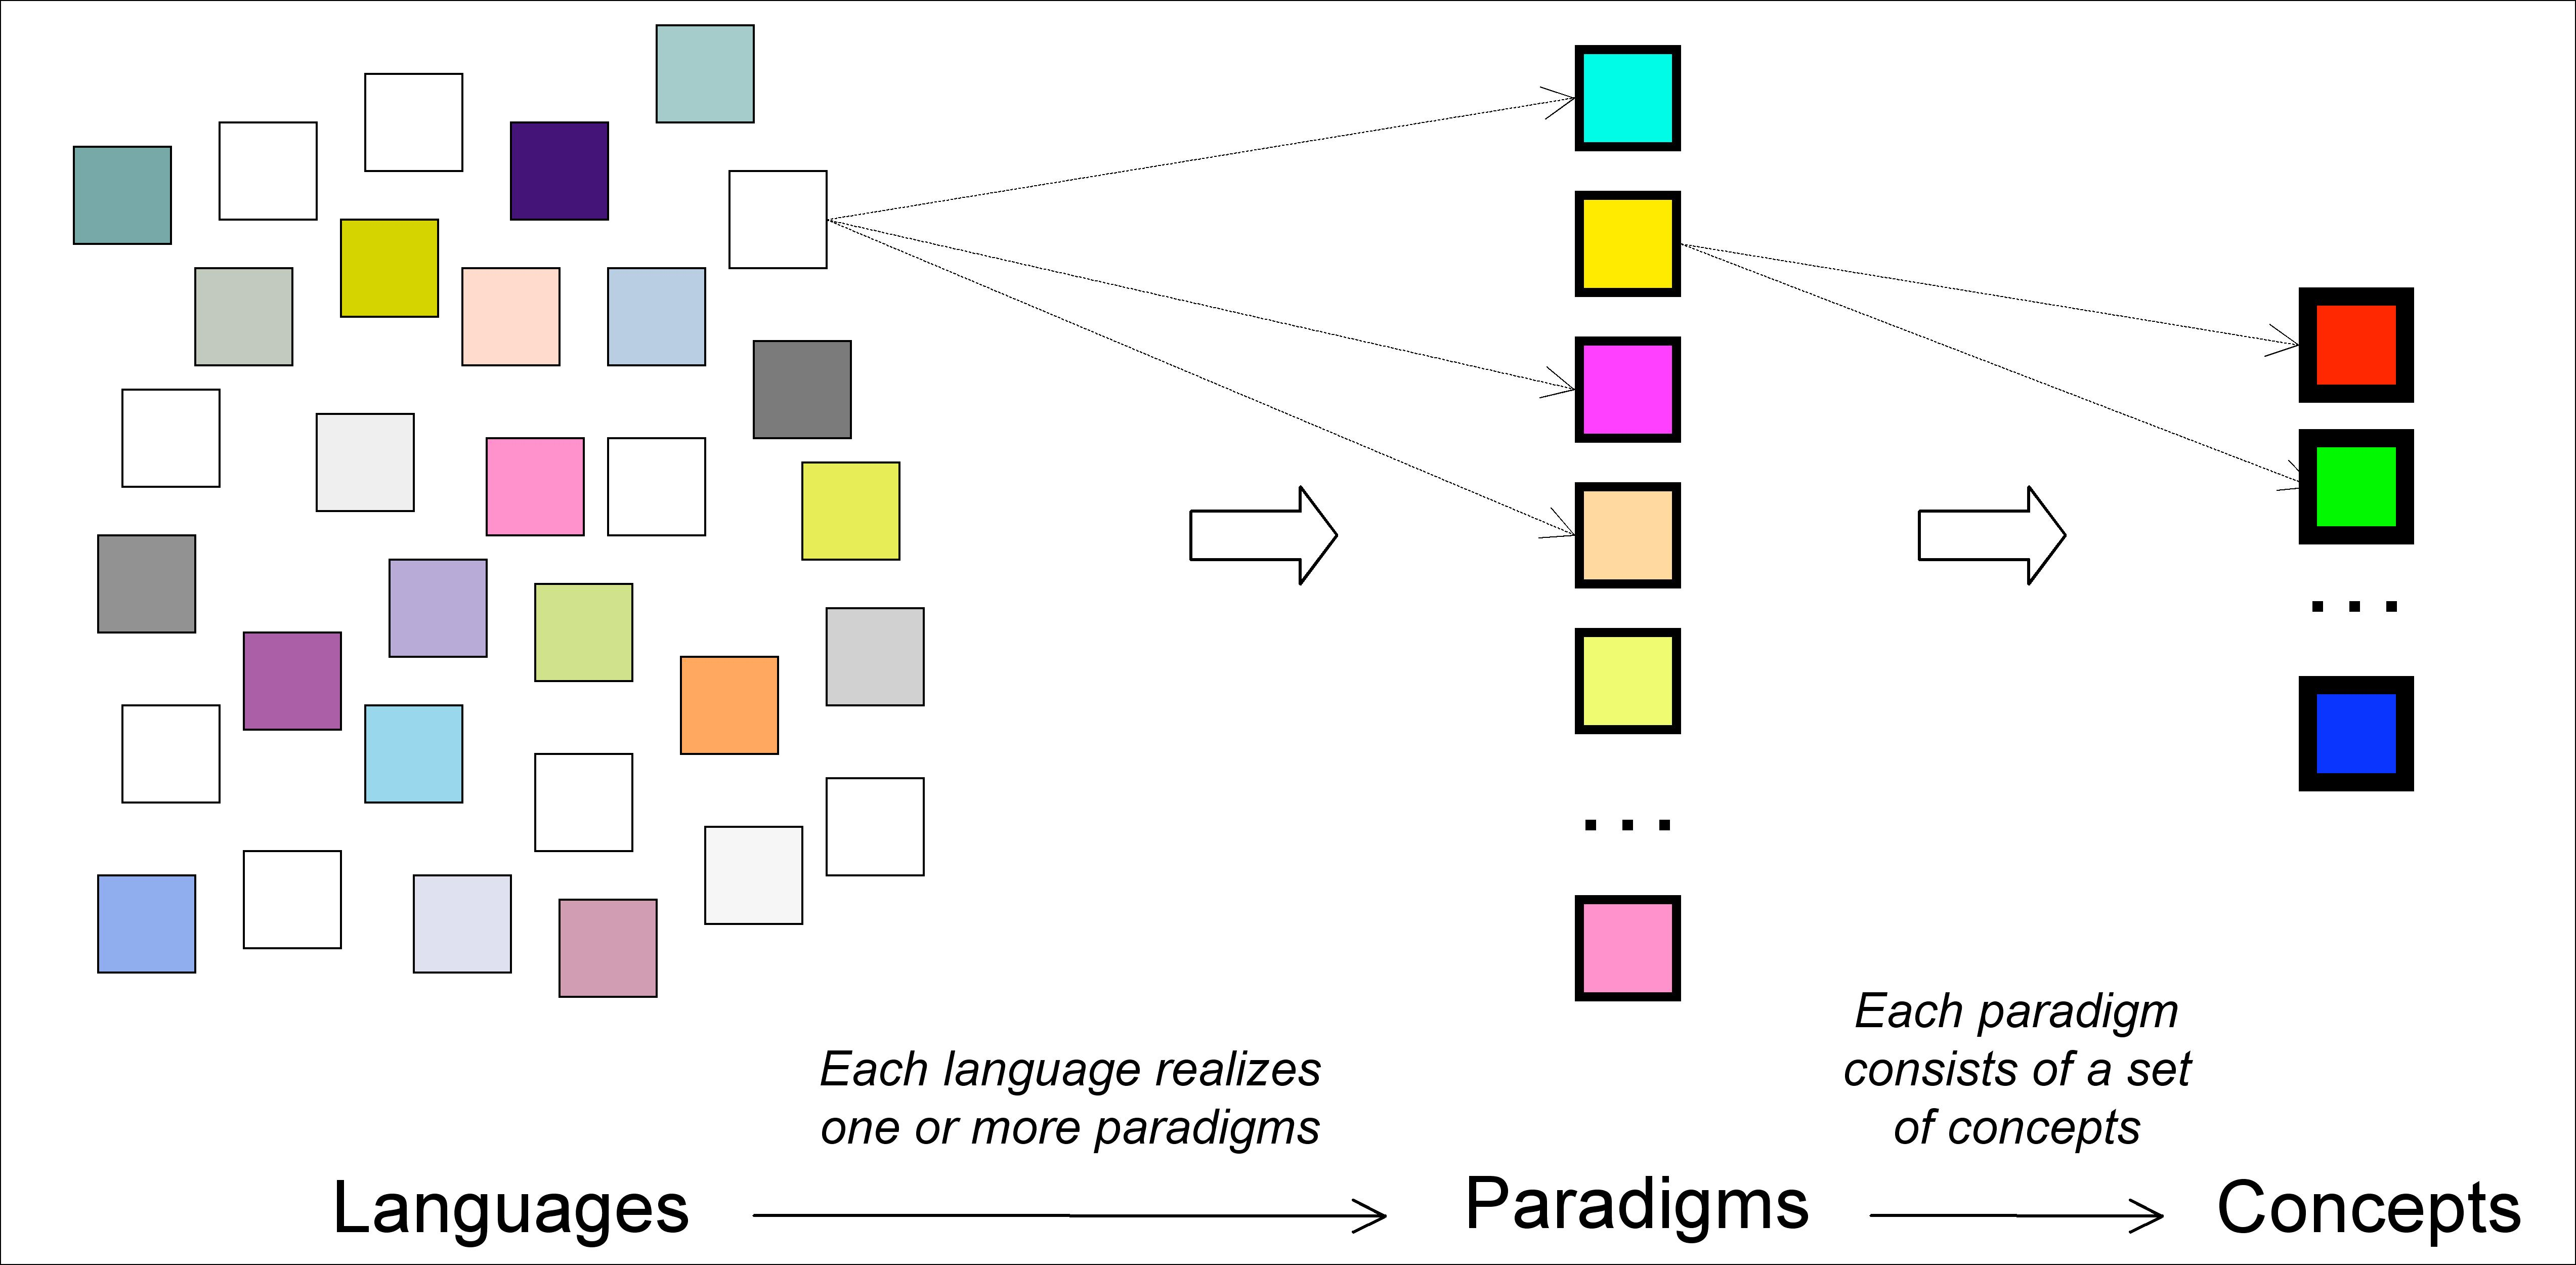
\includegraphics[width=12cm]{./fig/roy2009_languages_paradigms_and_concepts.jpeg}

  \small Fonte: \textcite[p.~12]{roy2009}.
  \label{img:LangsParadigmsConcepts}
\end{figure}

Da mesma forma que em engenharia de software (como um processo) pode-se adotar
diferentes metodologias de desenvolvimento, em linguagens de programação (como
modelos de computação) é desejável utilizar diferentes paradigmas de
programação.
Linguagens tradicionais como Java e C++ dão suporte a um ou dois paradigmas
diferentes.
“Isso é lamentável, pois problemas de programação diferentes precisam de
conceitos diferentes de programação para serem resolvidos claramente.”
\cite[p. 10]{roy2009}.

\textcite{roy2009} defende o uso de um modelo de programação \emph{multiparadigma},
porque:

\begin{citacao}
  Idealmente, uma linguagem deveria dar suporte a vários conceitos de forma
  bem integrada, para que o programador possa escolher os conceitos certos
  sempre que forem necessários, sem que um complique o outro.
  (p.~10; tradução nossa)
\end{citacao}

Apesar de linguagens tradicionais não dar suporte a esse modelo, entender os
conceitos certos pode melhorar a forma de programação, mesmo em linguagens que
não dê suporte direto a eles, assim como programação orientada a objetos é
possível em C com a atitude adequada \cite{roy2009}.

\textcite{roy2009} apresenta quatro modelos importantes que simplificam
programação concorrente em relação à linguagens convencionais: \emph{concorrência
declarativa}, \emph{programação funcional reativa}, \emph{programação síncrona
discreta}, e \emph{programação com restrições}.

No modelo declarativo de concorrência o resultado de um programa pode ser
calculado incrementalmente.
“Se a entrada de um programa concorrente é dada incrementalmente, então o
programa também irá calcular o resultado de saída incrementalmente.”
\cite[p. 238; tradução nossa]{roy2004}.
Esses paradigmas não possuem condições de corrida, \emph{‘race conditions’} em
inglês.
\todo{Esses últimos dois parágrafos parecem estar deslocados.}
\section{Programação de interfaces gráficas}
\label{sec:org5e54985}

\todo{Trecho vindo da introdução no corte de outubro de 2026, ainda por integrar a esta seção.}
Na implementação, a aplicação deixa de controlar a execução e se divide em
sub-rotinas que o \emph{toolkit} da interface chama quando o usuário age, e
programas assim parecem mais difíceis de organizar e modularizar
\cite[p. 79]{myers1994}.
Numa rede de \emph{callbacks}, a ordem em que os eventos chegam pode depender da
ordem em que os \emph{callbacks} foram registrados, o que a torna difícil de prever
\cite[p. 8]{blackheath2016}.
“Coordenar alterações ao estado compartilhado em meio a esse caos pode ser
desconcertante, e está longe de ser modular. A definição coloquial é \emph{Callback
Hell}.” \cite[p. 926; tradução nossa]{edwards2009}.
Em quatro sistemas de grande porte com as interfaces gráficas feitas na
mesma \gls{api}, \textcite[p. 770]{mijailovic2014} contaram de 1.221 a 31.285
tratadores de eventos.
Em 2026, o tratamento de eventos nas interfaces ainda se apoia em
\emph{callbacks} ou \emph{listeners}, que tornam difíceis de exprimir e de manter os
fluxos de interação complexos \cite[p. 8]{grolaux2026}.
As \emph{promises} têm semântica complexa, e o fluxo de controle e de dados do
código que as usa dificulta a compreensão e leva facilmente a erros
\cite[p. 162:1]{alimadadi2018}.

Conforme é notado por \textcite{blackheath2016}, a maioria das aplicações que
interagem com o ambiente externo são arquitetadas em torno de dois modelos de
programaçao, ou uma mistura dos dois:

\begin{description}
\item[{\emph{Threads}}] modelam transições de estado como um fluxo de controle.
Adequadas para operações de I/O ou qualquer situação onde as
transições de estado se enquadram em uma sequência claramente
definida.
\item[{Eventos}] são mensagens discretas e assíncronas que são propagadas pela
aplicação. Formam um modelo adequado para sequências menos
óbvias, principalmente onde as interações entre componentes são
mais complexas. Algumas aplicações incluem \emph{GUIs} e video
games.
\end{description}

Alguns problemas de computação são melhor resolvidos com o modelo baseado
em \emph{threads}. No entanto \textcite{blackheath2016} afirmam que a
abordagem com eventos geralmente é a melhor escolha.
\section{Programação funcional}
\label{sec:orgb2805f4}
\Gls{pf} é assim chamada porque sua operação básica é a
aplicação de funções à argumentos \cite{hughes1990}.
Lisp foi a primeira linguagem de programação funcional.
Criada em 1958 originalmente como uma notação matemática para programas de
computador, influenciada pelo \emph{cálculo lambda} de Alonzo Church.

Na matemática a ideia de \emph{quadrado de um número} pode ser expressa
algebricamente como uma função \(f(x)=x*x\).
Em Elm, \todo{Migrar os exemplos pra JavaScript.} a ideia de quadrado pode ser
expressa como \mintinline{elm}{quadrado x = x * x}.
A expressão pode ser lida em português da seguinte forma: “O quadrado de algo
é ele multiplicado por ele mesmo.”

A expressão algébrica denota uma função \(f\) que relaciona um número \(x\) com
seu quadrado, ou transforma \(x\) em seu quadrado.
A expressão em Elm define uma função \mintinline{elm}{quadrado} que transforma o
parâmetro \mintinline{elm}{x} em seu quadrado.
\textcite{roy2009} descreve uma função no contexto da \gls{pf}:

\begin{citacao}
  Funções são funções matemáticas: quando chamadas com os mesmos argumentos,
  elas sempre dão os mesmos resultados. Funções não mudam. No mundo real,
  as coisas são diferentes. Há poucas entidades reais que têm o comportamento
  intemporal das funções. Organismos crescem e aprendem. Quando o mesmo
  estímulo é dado à um organismo em momentos diferentes, a reação geralmente
  será diferente. (p. 26; tradução nossa)
\end{citacao}

Um programa funcional é uma expressão a ser avaliada, no contexto de um
conjunto de definições — principalmente definições de funções.
Por exemplo, dada as definições de função em \ref{code:programfnDefinitions}, um
programa pode consistir da expressão \mintinline{elm}{dobrar (somar 2 3)} e o resultado
do programa então seria \mintinline{elm}{10} \cite{noble1994}.

\begin{listing}[H]
  \centering
  \caption{Definição das funções \texttt{somar} e \texttt{dobrar}.}
  \begin{minted}[linenos=false]{elm}
    somar x y = x + y
    dobrar z = 2 * z
  \end{minted}
  \small Fonte: Adaptado de \textcite{noble1994}.
  \label{code:programfnDefinitions}
\end{listing}

Funções são consideradas \emph{cidadãs de primeira classe — do inglês ‘first-class
citizens’}, e podem ser passadas como argumentos da mesma forma que qualquer
outro tipo de dado.
Uma função é definida para ter um certo número de argumentos (sua \emph{aridade}),
mas se for calculada com menos argumentos o resultado é outra função.
Isso permite funções como as definidas em \ref{code:currying}, onde \texttt{inc} recebe
um número e adiciona \texttt{1} a ele, e \texttt{tres} aplica \texttt{f}, uma dada função, três
vezes à qualquer argumento em que \texttt{f} normalmente aceitaria, por exemplo: a
expressão \texttt{tres inc 2} resulta no valor \texttt{5} \cite{noble1994}.

\begin{listing}[H]
  \centering \caption{\emph{Currying}.}
  \begin{minted}[linenos=false]{elm}
    inc = somar 1
    tres f = f >> f >> f >>
  \end{minted}
  \small Fonte: Adaptado de \textcite{noble1994}.
  \label{code:currying}
\end{listing}
\subsection{Porque programação funcional é relevante}
\label{sec:org98a11ec}
Muitas das vezes as características e vantagens da programação funcional são
resumidas com declarações do tipo ‘programas funcionais não contêm
atribuições’, ‘não contêm efeitos colaterais’, e ‘não necessitam preescrever
o fluxo de controle’. Programação estruturada também já foi abordada de forma
similar: ‘programas estruturados não possuem \texttt{goto}, ‘blocos não
possuem múltiplos pontos de entrada e saída’. Essa analogia é feita por
\textcite{hughes1990} em \emph{Why Functinal Programming Matters}.

\textcite{hughes1990} comenta que “essas ‘vantagens’ da programação estruturada
são muito semelhantes em espírito as ‘vantagens’ da programação funcional”
(p. 3). O autor afirma que embora essas propriedades de programas
estruturados sejam úteis, elas não vão ao cerne da questão. Segundo o autor,
“a diferença mais importante entre programas estruturados e não-estruturados
é que programas estruturados são projetados de maneira modular”.

Modularidade é a chave para programação eficaz, no entanto ela é mais do que
separar um programa em módulos. \textcite{hughes1990} argumenta que “a
capacidade de se decompor um problema em partes depende diretamente da
capacidade de unir soluções” (p. 22). Hughes apresenta dois mecanismos
fornecidos por linguagens funcionais: \emph{funções de ordem superior} e
\emph{avaliação preguiçosa}. Estas \emph{ligas}, como são chamadas pelo autor, podem
contribuir significativamente para a modularização de programas:

\begin{citacao}
  Usando estas ligas pode-se modularizar programas de formas novas e úteis, e
  nós mostramos vários exemplos disso. Módulos menores e mais genéricos podem
  ser reutilizados mais largamente, aliviando programação posterior. Isso
  explica porque programas funcionais são menores e mais fáceis de escrever do
  que os convencionais. \cite[p.~22; tradução nossa]{hughes1990}
\end{citacao}
\section{Programação reativa}
\label{sec:org7b37cc8}
\todo{Trecho vindo da introdução no corte de outubro de 2026, ainda por integrar a esta seção.}
\textcite[p. 1-2]{bainomugisha2013} chamam as planilhas de “possivelmente a
linguagem de programação mais utilizada por usuários finais” (tradução nossa).
A maior parte da pesquisa em \gls{pr}, dizem ainda, descende do Fran, uma
linguagem da \gls{pf} do fim dos anos 1990.

No experimento de \textcite[p. 1125-1134]{salvaneschi2017}, 127 estudantes
do quarto ano de Ciência da Computação foram divididos ao acaso em dois
grupos, em duas rodadas.
Um grupo leu dez programas em Scala escritos com \gls{pr}, e o outro, os mesmos
programas com o \emph{Observer Pattern}.
Para cada programa, os participantes respondiam a uma pergunta de múltipla
escolha sobre o comportamento dele.
Só no grupo do \emph{Observer Pattern} os acertos acompanharam o nível de
habilidade de programação dos participantes.

Programação reativa abrange um leque enorme de conceitos de programação.
Isso se deve pela escolha da palavra ‘reativa’, que diz mais sobre uma
\emph{propriedade do que se programa} do que sobre um \emph{conceito de programação}.
Vários conceitos e paradigmas diferentes podem ser empregados na programação
de uma aplicação reativa — ou de qualquer tipo de programa \cite{roy2009}.
Entende-se então o porquê do paradigma abarcar tantos conceitos.
Portanto, faz sentido descrever \emph{programas reativos} e a propriedade
\emph{reativa}, antes de discutir os modelos de programação disponíveis para
abordá-los.
A \emph{priori}, é conveniente distinguir entre três tipos de programas de
computador:

\begin{itemize}
\item \emph{programa transacional}: computa resultados a partir de um conjunto de dados
de entrada. Compiladores e programas de computação numérica são alguns
exemplos clássicos;
\item \emph{programa interativo}: interage, no seu próprio ritmo, com usuários ou com
outros programas. Sistemas de tempo compartilhado são interativos, do ponto
de vista do usuário;
\item \emph{programa reativo}: também mantém interação contínua com seu ambiente, mas
no ritmo determinado pelo ambiente, não pelo próprio programa. Interfaces
gráficas\footnote{Este tipo de programa é popularmente conhecido como interativo — nota-se muito o
uso da expressão ‘Aplicações interativas’ por exemplo.} e robôs são exemplos muito comuns.
\end{itemize}

Programas interativos computam no seu próprio ritmo e tratam, em grande parte,
de comunicação.
Enquanto programas reativos só computam em resposta a demanda externa e lidam
principalmente com eventos ou interrupções de hardware \cite{berry1989}.
\emph{Interfaces gráficas} reagem a cliques do mouse, pressionamento de teclas,
gestos multitoque, etc.
\emph{Sistemas embarcados} reagem a sinais de hardware.
E \emph{programas de monitoração e controle} reagem a mudanças no ambiente externo
\cite{salvaneschi2015}.

Programação reativa é um paradigma que dá suporte à programação de aplicações
reativas através de alguns conceitos específicos.
Alguns deles são:

\begin{itemize}
\item \emph{fluxos de eventos\footnote{Tradução literal de \emph{‘event streams’}, em inglês.}}: servem para modelar notificações
discretas;
\item \emph{propagação automática de alterações}: o modelo de execução automaticamente
repercuti alterações nos dados;
\end{itemize}

\Gls{pr} é compartilha muitos conceitos com o paradigma de \gls{pfr}.
Os dois geralmente são confundidos na comunidade de praticantes.
\Gls{pfr} possui dois conceitos importantes que o diferencia da \gls{pr}.
O primeiro é o conceito de \emph{tempo contínuo} — na \gls{pr} o tempo é discreto.
O segundo é o conceito de \emph{semântica denotacional}.
\Gls{pfr} é mais indicada para domínios que precisam representar tempo contínuo,
como simulações físicas.
\Gls{pr} é mais indicada para sistemas reativos, como é explicado por
\textcite{roy2009}:

\begin{citacao}
  Usar tempo discreto simplifica enormemente a programação de sistemas reativos.
  Por exemplo, isso significa que subprogramas podem ser compostos de forma
  trivial: os eventos de saída de um subcomponente estão instantaneamente
  disponíveis como eventos de entrada para outros subcomponentes.
  (p. 36; tradução nossa)
\end{citacao}


% Estudos de Casos ---------------------------------------------------------
\chapter{Estudos de Casos}\label{chap:cases}
\section{Dimensões de avaliação}
\label{sec:org428c1d5}
\todo{Trecho vindo da introdução no corte de outubro de 2026, ainda por integrar a esta seção.}
\textcite[p. 58 e 60]{blackwell2019} registram, na psicologia da
programação, o pedido por ensaios controlados randomizados no estudo do
projeto de linguagens e o ceticismo sobre apoiar nesse empirismo um
processo de projeto complexo.
Para eles, a parte cognitiva das \glspl{dc} importa bem menos que a teoria de
projeto implícita nelas.

As outras duas, \emph{expressividade} e \emph{operações mentais difíceis}, vêm do grupo
que \textcite[p. 15]{kiss2014} deixou de fora e que, a seu ver, teria
sido útil se as linguagens e os \emph{toolkits} comparados fossem muito mais
diferentes.
Na comparação principal, \textcite[p. 11-12]{kiss2014} escolheu o
ScalaFX porque este envolve o próprio JavaFX e porque o Scala é
sintaticamente próximo do Java.
Aqui, cada tecnologia traz as próprias abstrações, e as três notações
diferem na forma de escrever a coordenação.
E, ao avaliar bibliotecas reativas, ele próprio descreve o esforço
mental de cada uma sem uma dimensão para isso
\cite[p. 87 e 97]{kiss2014}.

As duas tratam da leitura do código.
A expressividade é a facilidade de reconhecer o propósito de cada
trecho, e as operações mentais difíceis obrigam quem lê a contar nos
dedos ou anotar à parte para acompanhar o que acontece \cite{green1996d}.
Ao avaliar se quem lê entende uma especificação,
\textcite[p. 267]{britton2001} também as incluíram entre as dimensões
especialmente úteis.
Na comparação de \textcite{mernik2009} entre o \gls{xaml} e o C\# Forms, as duas
estiveram entre as dimensões que mais pesaram na compreensão dos
programas.

As outras três do grupo ficam de fora.
O compromisso prematuro nasce da ordem em que o ambiente obriga a
construir o programa, e o código pronto não guarda essa ordem
\cite{green1996d}.
A consistência mede o quanto quem aprende consegue adivinhar da notação,
e só se avalia por introspecção \cite{green1996d}.
Já a notação secundária (comentários, indentação e nomes) é própria de
quem escreve \cite{green1996d}.
Aqui, ela é padronizada entre as tecnologias, e por isso não distingue
uma notação da outra.
As dimensões utilizadas neste trabalho são baseadas nas \glspl{dc} de
\textcite{green1989}. Assim usamos critérios estabelecidos, o que facilita a
comparação de nossos resultados com trabalhos baseados nas \glspl{dc}. O \emph{framework}
completo possui 14 dimensões, mas os autores recomendam usar um subconjunto
apropriado para o artefato em mãos.

\begin{description}
\item[{Nível de abstração}] \emph{Disponibilidade e tipos de mecanismos de abstração}

O sistema fornece alguma forma de definir novos termos com a notação pra
que eles possam ser extendidos afim de descrever ideias claramente? Os
detalhes podem ser encapsulados? O sistema insiste em definir novos
termos? Qual o número de novos conceitos de alto nível devem ser
aprendidos pra se fazer uso do sistema? Eles são fáceis de aprender e
usar?

   Cada novo conceito é um empecilho pra aprendizagem e aceitação, mas
também pode tornar um código complexo mais compreensível. Por exemplo, o
React emprega o \emph{fluxo de dados de mão única} --- do inglês \emph{one-way data
flow} ou \emph{one-way binding} --- em sua arquitetura. É necessário aprender
conceitos novos para usar os componentes do React de forma adequada. Não
compensa para aplicações pequenas, mas para aplicações complexas pode tornar
o código mais compreensível e passível de manutenção porque os detalhes
podem ser encapsulados em novos termos: os componentes.

Outro exemplo é a função:

\begin{citacao}
  A function has a name and, optionally, parameters as well as a body that
  returns a value following certain computational steps. A client can simply
  refer to a function by its name without knowing its implementation details.
  Accordingly, a function abstracts the computational process involved in the
  computation of a value. The learning barrier to the principle of a function is
  not great but it can still make a lot of code much more understandable 3 by
  hiding unimportant details.
  \cite[p.~13]{kiss2014}
\end{citacao}

\item[{Proximidade de descrição}] \todo{Traduzido de “Closeness of mapping”, poderia ser “Proximidade de mapeamento”} \emph{Semelhança entre representação e o domínio}

O quão relacionado é a notação com o resultado que ela descreve, ou
melhor, o domínio do problema? Que partes parecem ser uma forma
particularmente estranha de descrever algo?

\begin{citacao}
  Um exemplo é a definição de layout de uma interface gráfica. Linguagens que
  não fornecem uma forma de descrever o layout de modo aninhado, ou seja,
  hierárquico, e como tal força o programador a “linearizar” o código com o uso
  desnecessário de variáveis intermediárias, dificultando enchergar como a
  estrutura de definição do layout corresponde com o layout final da aplicação.
  Não é atoa que especificações baseadas no XML são amplamente usadas na
  construção de interfaces gráficas em linguagens sem suporte nativo para
  representação hierárquica de layout.
  \cite[p.~13; tradução nossa]{kiss2014}
\end{citacao}

\item[{Dependências ocultas}] \emph{Vínculos importantes implícitos entre entidades}

As dependências entre as entidades da notação são visíveis ou ocultas?
Todas as dependências são especificadas em ambas as direções? Alterações
locais podem ter efeitos globais confusos?

Se uma entidade cita outra, que por sua vez cita uma terceira, a
alteração do valor da terceira entidade pode desencadear efeitos
inesperados. O principal problema não é o fato de A depender de B, mas sim
que a dependência não é explicitamente visível. Um caso bem conhecido de dependência
oculta é o “problema da classe base frágil”\footnote{Veja: \url{https://en.wikipedia.org/wiki/Fragile\_base\_class}.}.

\begin{citacao}
  In (complex) class hierarchies a seemingly safe modification to a base class
  may cause derived classes to malfunction. The IDE in general cannot help
  discovering such problems and only certain programming language features can
  help preventing them. Another example are non-local side-effects in
  procedures, i.e. the dependencies of a procedure with non-local side-effects
  are not visible in its signature.
  \cite[pg.~14]{kiss2014}
\end{citacao}

\item[{Propensão a erros}] \emph{Notação incita erros}

Até que ponto a notação influência o programador a cometer um erro? Fazer
algumas coisas parece ser particularmente complexo ou difícil, p. ex.,
juntar várias coisas?

Em muitas linguagens dinâmicas com definições implícitas de
variáveis\footnote{Isto é, quando não se precede uma definição de variável
com \texttt{var} ou \texttt{let} por exemplo.}, um erro de tipagem em uma variável pode
de repente causar erros difíceis de encontrar já que o \gls{ide} nem sempre
pode apontar tal erro devido a dinamicidade na linguagem. A inicialização
implícita de variáveis com valor \texttt{null} pode levar a uma exceção de
ponteiro nulo se o programador esquecer de inicializar as variáveis
corretamente antes de usá-las.

\item[{Concisão        }] \emph{Verbosidade da linguagem}

Quantos símbolos ou quanto espaço a notação requer pra produzir um certo
resultado ou expressar uma ideia. Que tipos de coisas ocupam mais espaço
para se descrever?

\begin{citacao}
  Some notations can be annoyingly long-winded, or occupy too much valuable
  “real-estate” within a display area. In Java before version 8 in order to
  express what are lambdas today anonymous classes were employed. Compared to
  Java 8’s lambdas these anonymous classes used to be a very verbose way of
  encoding anonymous functions especially when used in a callback-heavy setting
  like traditional GUI programming~\cite[p.~14]{kiss2014}.
  \todo[inline]{Pensar num exemplo mais próximo da Web e substituir citação direta.}
\end{citacao}

\item[{Viscosidade    }] \emph{Resistência a mudanças}

Existe alguma barreira contra mudança na notação? Quanto esforço é
necessário pra fazer uma alteração num programa expresso na notação?

Num sistema viscoso o usuário precisa realizar várias passos para
concluir uma tarefa. Alterar o tipo de retorno de uma função pode causar
erros em várias partes do código onde a função é chamada. Nesses casos um
\gls{ide} pode ajudar muito.
\end{description}


Outras dimensões que ficaram de fora são:

\begin{itemize}
\item Comprometimento prematuro: \emph{limitações na ordem de fazer as coisas}
\item Expressividade: \emph{o propósito de uma entidade pode ser rapidamente determinado}
\item Consistência: \emph{semânticas parecidas são apresentadas em estilo sintático
parecido}
\item Operações mentais difíceis: \emph{alto esforço cognitivo pra realizar tarefas}
\item Notação secundária: \emph{informações extras por meio de notações além das
formais}
\end{itemize}
\todo[inline]{Berndt sugeriu considerar “Expressividade” e “Operações mentais difíceis”.}

Em outras situações, e dependendo dos artefatos de informação, essas dimensões
poderiam ser úteis. Se tivéssemos focado mais nas ferramentas e no processo de
construção dos estudos de caso então as seguintes dimensões poderiam ser usadas:

\begin{itemize}
\item Visibilidade: \emph{habilidade de ver os componentes claramente}
\item Análise progressiva: \emph{trabalho realizado pode ser verificado em qualquer
momento}
\item Provisoriedade\todo{'momentaneidade' ou 'transitoriedade'}: \emph{grau
de comprometimento com uma ação ou marco}
\end{itemize}
\section{*Revisão do JavaScript}
\label{sec:org8b6f50e}
Talvez devêssemos colocar uma seção de revisão das ferramentas utilizadas na
implementação dos estudos de caso? Poderíamos descrever os recursos relevantes
para nossa análise.
\todo[noline]{Berndt disse p/ colocar como apêndice}
\section{Processamento de listas}
\label{sec:org59a4e3e}

Uma coleção é um agrupamento com uma quantidade variável de itens, que (1)
compartilham algum significado ao problema a se resolver e (2) precisam ser
manipulados juntos de forma controlada.

O único tipo de coleção no JavaScript é o arranjo, ou \emph{array}, que pode ser
construído através do objeto\footnote{Diferente da maioria das linguagens, em que objetos são
instâncias de classes, no JavaScript os objetos são extensões de \emph{protótipos}.} global \mintinline{js}{Array}, ou da
notação de arranjos literais com colchetes:

\begin{listing}[htbp]
\caption{Criando coleções}
\begin{minted}[]{js}
var collection1 = new Array();
var collection2 = [];
\end{minted}
\end{listing}

Uma tarefa muito comum na programação é a iteração\footnote{O processo de percorrer, um por um, os itens de uma coleção.} de coleções.
Um mecanismo muito utilizado para tal é o comando \mintinline{js}{for}. Em
\ref{code:forLoopTraverse} é demonstrado o uso do comando \mintinline{js}{for} para
percorrer os itens da coleção \mintinline{js}{people} e mostrar cada um no console de
depuração.

\begin{listing}[htbp]
\caption{\label{code:forLoopTraverse}Percorrendo uma coleção com o laço \mintinline{js}{for}}
\begin{minted}[]{js}
var people = ["Alan Turing", "Alonzo Church", "Kurt Gödel"];
var count  = 0;

for (count = 0; count < people.length; count++) {
  console.log(people[count]);
}
\end{minted}
\end{listing}
\subsection{Formatação de preços}
\label{sec:org83eb487}

Nesta seção veremos como formatar uma lista preços para serem mostrados na
tela, p. ex., transformando um valor numérico \mintinline{js}{50.45} em uma \emph{string}
\mintinline{js}{"R$ 50.45"}. Para isso usamos uma função de formatação que é aplicada
a cada valor da lista. A função de formatação pode ser observada em
\ref{code:formatPriceFunction}.

\begin{listing}[htbp]
\caption{\label{code:formatPriceFunction}Função pra formatar um preço}
\begin{minted}[]{js}
function formatPrice(price) {
  return 'R$' + price.toFixed(2);
}
\end{minted}
\end{listing}

Em \ref{code:formatPricesFor} pode-se ver a solução implementada com o laço
\mintinline{js}{for}.

\begin{listing}[htbp]
\caption{\label{code:formatPricesFor}Formatação de preços com laço \mintinline{js}{for}}
\begin{minted}[]{js}
const prices = [50.45, 47, 20.99, 3.44, 1];
let formatedPrices = [];

for (let i = 0; i < prices.length; i++) {
  formatedPrices.push(formatPrice(prices[i]));
}
\end{minted}
\end{listing}

Em \ref{code:formatPricesMap} pode-se ver a solução implementada com a função
\mintinline{js}{map}.

\begin{listing}[htbp]
\caption{\label{code:formatPricesMap}Formatação de preços com laço \mintinline{js}{for}}
\begin{minted}[]{js}
const prices = [50.45, 47, 20.99, 3.44, 1];

const formatedPrices = prices.map(formatPrice);
\end{minted}
\end{listing}

Outras ideias:

\begin{itemize}
\item Adicionar \(1\) a cada número de uma lista
\item Multiplicar os números de uma lista
\item Transformar palavras com letras minúsculas de uma lista em palavras com
letras maiúsculas
\end{itemize}
\subsection{Seleção de valores com \texttt{filter()}}
\label{sec:org21851ae}
Remover nomes que não começam com ‘S’
\subsection{Nivelamento de valores com \texttt{concatAll()}}
\label{sec:orgc1e2101}
\subsection{Redução de valores com \texttt{reduce()}}
\label{sec:orgd381346}

O método \mintinline{js}{reduce()} executa uma função \textbf{reducer} para cada item da
lista, resultando num único valor. Em \ref{code:somaDePreçosComReduce} é
demostrado a soma dos preços de uma lista usando o método \mintinline{js}{reduce()}.
Nesta demonstração a função \mintinline{js}{somar()} é o \textbf{reducer}.

\begin{listing}[htbp]
\caption{\label{code:somaDePreçosComReduce}Soma dos preços de uma lista com o método \mintinline{js}{reduce()}.}
\begin{minted}[]{js}
const preços = [50.45, 47, 20.99, 3.44, 1];

const somar = (a, b) => a + b;
const total = preços.reduce(somar);
\end{minted}
\end{listing}
\subsection{Agrupamento de valores com \texttt{zip()}}
\label{sec:orgdaad8c5}
\section{Coordenação de eventos}
\label{sec:org66d03a1}
\todo{Trecho vindo da introdução no corte de outubro de 2026, ainda por integrar a esta seção.}
Cada pesquisa de uso tem um limite de amostra.
Os respondentes do Stack Overflow Developer Survey 2025 são recrutados
sobretudo pelos próprios canais do site, o que favorece os usuários mais
ativos \cite{stackoverflow2025}.
No W3Techs, basta achar a biblioteca em qualquer página para o \emph{site}
contar, o que favorece o jQuery e nada diz das aplicações novas
\cite{w3techs2026,w3techs2026a}.
O State of JS 2025 é um levantamento aberto a quem quiser responder, que se
declara o retrato de um subconjunto de desenvolvedores \cite{devographics2026}.
Na Pesquisa Código Fonte TV 2026, cada participante escolhe uma só
ferramenta, entre 130 de todas as áreas, o que encolhe as fatias, e a
audiência do canal que a divulga tende a estar super-representada
\cite{codigofonte2026}.
O W3Techs nem separa o Angular do AngularJS, antecessor dele e sem
suporte desde 2022 \cite{thompson2022}; a Pesquisa Código Fonte TV os
separa e dá 571 participantes ao Angular e 78 ao AngularJS
\cite{codigofonte2026}.

O jQuery e o Web Component derivam a Lista filtrável com \texttt{filter}, \texttt{sort} e
\texttt{map}, funções de \gls{pf}.
E o React e o Solid recorrem a efeitos para sincronizar o componente com
sistemas externos, como o armazenamento do navegador no Carrinho.
A documentação do React chama os efeitos de “uma saída de emergência do
paradigma do React” \cite[tradução nossa]{meta2026b}.

Três das cinco tarefas partem do 7GUIs \cite[p. 17, 25 e 34]{kiss2014}:

\begin{description}
\item[{Contador}] a tarefa \emph{Counter};
\item[{Formulário com validação}] a \emph{Flight Booker}, ampliada com os campos de
um formulário real;
\item[{Lista filtrável}] o filtro por prefixo da tarefa \emph{Crud}.
\end{description}

O \emph{Timer} trata da concorrência entre um relógio e o usuário, mas nenhuma
das sete tarefas faz uma requisição cujas respostas chegam fora de ordem ou
são canceladas \cite[p. 30]{kiss2014}.
E nenhuma põe três componentes independentes para ler e alterar o mesmo
estado, como os do Carrinho.

No React, um valor derivado é uma expressão comum, recalculada a cada
execução do componente \cite{meta2026b}.
No Solid, é uma função que lê o \emph{signal} \cite{solidjs2026a}.

No Android, as duas variantes são escritas em Kotlin, a linguagem que o
Android recomenda e a única em que o Compose se escreve \cite{android2026a}.
O porte do domínio para Kotlin responde diferente em entradas-limite, como
anos de 0 a 99, e cada diferença conhecida fica registrada num teste.
Entre Views e Compose, a única diferença admitida nas capturas é a de
poucos pixels na renderização do texto.
\subsection{Contador}
\label{sec:org06896ae}

\begin{description}
\item[{Problema}] entender os conceitos essenciais da linguagem e a estrutura
básica necessária
\end{description}

\begin{figure}[htbp]
\caption{\label{img:contador}Interface gráfica do Contador.}
\centering
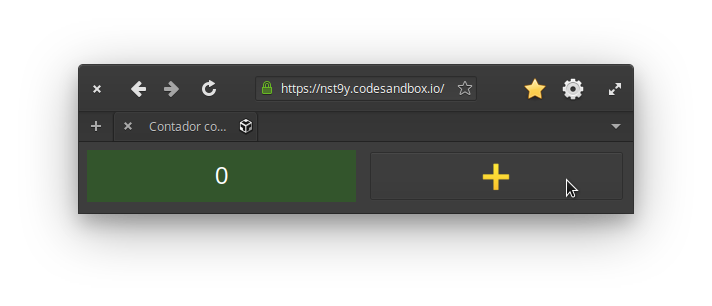
\includegraphics[width=12cm]{./fig/screenshot-contador-epiphany.png}
\end{figure}

A implementação do contador usando classes poder ser observado em
\ref{code:contadorComPOO}.

\begin{listing}[htbp]
\caption{\label{code:contadorComPOO}Contador com POO.}
\begin{minted}[]{js}
// No Java isto extenderia alguma classe padrão do toolkit,
// como `Application`
class Contador {
  constructor(props) {
    // Em Java estas propriedades precisam ser definidas antes
    this.contador = props.valorInicial;
    this.caixaDoValor = document.getElementById("valor");
    this.botãoDeIncrementar = document.getElementById("botãoDeIncrementar");
    this.botãoDeIncrementar.addEventListener(
      "click",
      // Isto requer uma explicação um tanto extensa
      this.tratarClique.bind(this)
    );
  }

  tratarClique(_evento) {
    this.contador = this.contador + 1;
    this.renderizar();
  }

  // Equivalente ao `public static void main()` do Java
  renderizar() {
    this.caixaDoValor.innerText = this.contador;
  }
}

const contador = new Contador({ valorInicial: 0 });
// Como no Java o `main()` é padronizado, sua execução seria
// feita automaticamente pelo ambiente de execução.
contador.renderizar();
\end{minted}
\end{listing}

O \mintinline{js}{tratarClique.bind(this)} na linha 12 requer uma explicação um tanto
extensa.

O contador usando função e operadores do xstream pode ser observado em
\ref{code:contadorComPR}.

\begin{listing}[htbp]
\caption{\label{code:contadorComPR}Contador com PR.}
\begin{minted}[]{js}
import fromEvent from "xstream/extra/fromEvent";

const Contador = props => {
  const caixaDoValor = document.getElementById("valor");
  const botãoDeIncrementar = document.getElementById("botãoDeIncrementar");

  // Fluxo que emite um evento toda vez que o botão for clicado
  const cliqueStream = fromEvent(botãoDeIncrementar, "click");

  // Fluxo que emite "valor + 1" (acumulado) toda vez que
  // cliqueS emite um evento
  const contadorStream = cliqueStream.fold(
    (valor, _evento) => valor + 1,
    props.valorInicial
  );

  const observador = {
    next: valor => {
      caixaDoValor.innerText = valor;
    }
  };

  contadorStream.addListener(observador);
};

Contador({ valorInicial: 0 });
\end{minted}
\end{listing}
\subsubsection{Análise}
\label{sec:org7c53d47}

Essa primeira análise é focada no básico.
\paragraph{Nível de abstração}
\label{sec:org6eb73aa}
Na solução com \gls{poo} os conceitos da linguagem que deve-se entender são:
classes, construtor, objetos, propriedades, métodos, \emph{callbacks} na forma
de método, e conhecimento da \gls{api} do objeto do documento do \gls{html} ---
\gls{dom}.
Além do caso do \mintinline{js}{this} específico do JavaScript:
\mintinline{js}{this.tratarClique.bind(this)}.
Embora sejam conceitos básicos para um programador experiente em JavaScript
e \gls{poo}, o número é grande.
Abstrações mais sofisticadas não são necessários pelo Contador e o sistema
não insiste em abstrações especiais.
Apesar da solução usar uma quantidade considerável de conceitos, eles são
básicos, então observamos que o Nível de Abstração é baixo, ou seja, bom.

Em contrapartida, na solução com \gls{pr} os conceitos usados são: funções,
variáveis, fluxos e eventos, callbacks, e a \gls{api} do \gls{dom}.
A abstração mais sofisticada é o método \mintinline{js}{fold()} do fluxo de evento,
que nada mais é que uma versão assíncrona do \mintinline{js}{Array.reduce()}
nativo --- veja a soma de preços em \ref{code:somaDePreçosComReduce}.
Ambos produzem um resultado para cada elemento da lista.
A diferença é que no primeiro a lista é de eventos assíncronos, e infinita.
No segundo a lista é síncrona, com valores escales (números, \emph{strings},
objetos, etc.).
\todo{Paralelo entre métodos assíncronos e síncronos em outra seção?}
Níveis mais altos de abstração não são necessários, então a solução com \gls{pr}
é igualmente boa ou um pouco melhor que a solução com \gls{poo} quanto ao Nível
de Abstração.
\paragraph{Proximidade de descrição}
\label{sec:org0e2e10a}
Essa dimensão/critério faz mais sentido para análise de apresentação do que
comportamento (coordenação de eventos).
\paragraph{Dependências ocultas}
\label{sec:orgf171659}
\todo[noline]{Acredito que o HTML só não está situado no mesmo local que o código JavaScript, que é diferente de “oculto”.}
As únicas dependências que podem ser consideradas ocultas são os elementos
\gls{html} buscados pelo identificador com \texttt{document.getElementById("id")}.
\paragraph{Propensão a erros}
\label{sec:org63ff66f}
Na solução com \gls{poo}, esquecer de vincular a instância do contador à função
\texttt{tratarClique()} resultará no erro “TypeError: this.renderizar is not a
function”.
Pois o valor do \texttt{this} estará vinculado ao objeto que chamou
\texttt{tratarClique()}, ou seja, o \texttt{this.botãoDeIncrementar}.
\todo{Talvez isso seja uma dependência oculta?}
Isso se deve ao fato de a palavra chave \texttt{this} se comportar de forma
diferente no JavaScript quando comparado com outras linguagens.

\begin{quote}
In most cases, the value of this is determined by how a function is called
(runtime binding). It can't be set by assignment during execution, and it
may be different each time the function is called. ES5 introduced the
bind() method to set the value of a function's this regardless of how it's
called, and ES2015 introduced arrow functions which don't provide their own
this binding (it retains the this value of the enclosing lexical context).
\cite{This2020}.
\end{quote}

\todo[inline]{Nos próximos exemplos acredito que podemos usar as funções de seta
  como callback no lugar dos métodos, pois possuem o valor do this vinculado
  lexicalmente. O Java possui lambdas desde a versão 8, o que despensa o uso de
  métodos para casos como esse. Ou já removemos desse primeiro? Pra evitar ter
  que explicar o \texttt{.bind(this)} que é um problema específico do
  JavaScript}.

Na solução com \gls{pr}, esquecer de definir o observador fará com que a
\texttt{caixaDoValor} não seja atualizada.
Pois ela não será renderizada, apesar de toda a lógica do contador
funcionar.
Apesar de tudo, essas possibilidades de erros não são críticas.
\paragraph{Concisão}
\label{sec:org785ebc6}
Na solução com \gls{poo} o método \mintinline{js}{tratarClique()}, usado como \emph{callback},
poderia ser substituído por uma função de seta.
Além de poupar algumas linhas o uso do \mintinline{js}{.bind(this)} se torna
desnecessário.
Veja o código do Contador com \gls{poo} e função de seta em
\ref{code:contadorComPOOeFuncDeSeta} no apêndice.
Na solução com \gls{pr} a variável intermediária \mintinline{js}{contadorStream} poderia ser
removida, encadeando a chamada do \mintinline{js}{fromEvent} com o \mintinline{js}{fold()}:
\mintinline{js}{const cliqueStream = fromEvent().fold()}.
No entanto essa manobra diminuiria a legibilidade do
código\footnote{Note que o nome da variável \mintinline{js}{cliqueStream} já nem faz mais
sentido, pois o resultado da expressão não inclui apenas os eventos de clique.}.
De qualquer forma, a \gls{pr} evita a verbosidade da declaração da classe e dos
métodos, além da repetição do \mintinline{js}{this}.
Então em termos de Concisão a \gls{pr} está à frente da \gls{poo}.
\paragraph{Viscosidade}
\label{sec:org7ca5a61}
Num caso tão simples como o do Contador a única resistência a alteração
está em renomear atributos no caso da \gls{poo}, e variáveis na \gls{pr}.
No entanto isso é inevitável ao renomear termos.
Além disso o \gls{ide} pode ajudar através de uma funcionalidade de refatoração.
\todo{Talves seja interessante analisar a viscosidade da alteração pra colocar um botão de decremento (-1) do Contador.}
\subsection{Reserva de voo}
\label{sec:orgd294180}


\chapter{Resultados}\label{chap:results}
Resultados aqui…

\todo{Trecho vindo da introdução no corte de outubro de 2026, ainda por integrar a esta seção.}
Na tabela-síntese, cada célula traz um juízo curto e a tarefa de que vem a
evidência.
Quando o Solid e o Angular com \emph{signals} divergem numa \gls{dc}, a célula o
registra.
A seção de cada \gls{dc} cita as outras tarefas quando contradizem a escolhida, e a tabela
diz "sem diferença" quando nenhuma tarefa mostra uma.
A contagem de linhas inclui a estrutura da tela, esteja ela no mesmo arquivo da
coordenação ou num arquivo à parte, como o \gls{html} da página no jQuery e o
layout \gls{xml} nas Views.


% Conclusão ----------------------------------------------------------------
\chapter{Conclusão}\label{chap:conclusion}
Blá blá blá…
\section{Considerações finais}
\label{sec:org5e03da1}
\todo{Trecho vindo da introdução no corte de outubro de 2026, ainda por integrar a esta seção.}
Uma forma de conferir o juízo de quem avalia é colher o dos usuários, como no
estudo de \textcite[p. 1512-1513 e 1519]{zimmerle2025}, em que 12 estudantes
responderam, depois das tarefas, a 24 afirmações agrupadas em cinco
dimensões derivadas das \glspl{dc}.



%------------------------------------------------------------- REFERÊNCIAS %

\cleardoublepage

%\nocite{*}                  % para incluir referências não citadas no texto

\printbibliography[heading=bibintoc,title=REFERÊNCIAS]


% https://www.diferenca.com/anexo-e-apendice/
% --------------------------------------------------------------- APÊNDICES %
\apendices{}

\chapter{Variações dos Estudos de Caso}
\label{apend:1}

\begin{listing}[htbp]
\caption{\label{code:contadorComPOOeFuncDeSeta}Contador com POO e função de seta.}
\begin{minted}[]{js}
class Contador {
  constructor(props) {
    this.contador = props.valorInicial;
    this.caixaDoValor = document.getElementById("valor");
    this.botãoDeIncrementar = document.getElementById("botãoDeIncrementar");

    const tratarClique = _evento => {
      this.contador = this.contador + 1;
      this.renderizar();
    };
    this.botãoDeIncrementar.addEventListener("click", tratarClique);
  }

  renderizar() {
    this.caixaDoValor.innerText = this.contador;
  }
}

const contador = new Contador({ valorInicial: 0 });
contador.renderizar();
\end{minted}
\end{listing}
\chapter{Etapas da revisão bibliográfica}
\label{apend:2}

A revisão bibliográfica, por palavras-chave e \textit{snowballing}
\cite[p.~3-4]{wohlin2014}, teve duas rodadas, em setembro e outubro de
2026, no OpenAlex, no Crossref, na ACM Digital Library, na IEEE Xplore, na
SBC-OpenLib e na \gls{bdtd}.
Entram trabalhos revisados por pares e, da \gls{bdtd}, dissertações e
teses, em inglês ou português, de três tipos.
Os primeiros tratam de \gls{pr} ou da programação declarativa de interfaces
gráficas.
Os segundos comparam a compreensão e a usabilidade de uma ou de outra com
as dos \textit{callbacks} ou do \textit{Observer Pattern}.
Os terceiros aplicam as \glspl{dc} a linguagens e bibliotecas.
O \textit{snowballing} para a frente parte de dez trabalhos centrais e, na
segunda rodada, percorre todos os citantes de quatro deles em duas
iterações; uma terceira, parcial, vê as referências de um trabalho e os que
citam o 7GUIs, e não traz trabalho novo.
Para trás, percorre as referências de dois trabalhos.
A revisão não viu os citantes de \textcite{kiss2014}, que o OpenAlex não
indexa, e julgou só pelo título 280 registros sem resumo.

Entre os trabalhos incluídos, os mais próximos deste aplicam as \glspl{dc}
a linguagens e bibliotecas de interface ou de \gls{pr}:
\textcite{mernik2009} comparam o \gls{xaml} e o Windows Forms em C\#,
\textcite{kiss2014} compara JavaFX, ScalaFX, Scala.Rx, ReactFX e Elm, e
\textcite{zimmerle2025} avaliam o RxJS e o Bacon.js.
\textcite{grolaux2026} comparam, sem as \glspl{dc}, o \textit{async} e
\textit{await} com outras formas de tratar os eventos de interface.
Nenhum trabalho incluído avalia pelas \glspl{dc} a notação do React nem a
do Solid e do Angular com \textit{signals}, nem compara as três notações
nas mesmas tarefas; essa é a lacuna que a introdução declara.

As tabelas a seguir dão os números de cada etapa das duas rodadas.

\begin{table}[htbp]
\centering
\caption{\label{tab:revisaoRodada1}Primeira rodada (24 de setembro de 2026).}
\small
\begin{tabular}{p{0.55\textwidth}p{0.35\textwidth}}
\hline
Etapa & Registros \\
\hline
Buscas por palavras-chave (19 consultas) & 301 resultados \\
\textit{Snowballing} para a frente (10 trabalhos) & 359 citantes, de 932, com sobreposição \\
\textit{Snowballing} para trás (1 trabalho) & 82 referências \\
Títulos únicos triados & cerca de 530 \\
Lidos no resumo & cerca de 40 \\
Incluídos & 23 \\
\hline
\end{tabular}

Fonte: o autor.
\end{table}

\begin{table}[htbp]
\centering
\caption{\label{tab:revisaoRodada2}Segunda rodada (2 de outubro de 2026).}
\small
\begin{tabular}{p{0.55\textwidth}p{0.35\textwidth}}
\hline
Etapa & Registros \\
\hline
Citantes de 4 trabalhos, todos os anos & 2.359, com sobreposição \\
Citantes únicos desde 2013 & 1.230, dos quais 263 já vistos e 280 sem resumo \\
Iteração 1, incluídos por título e resumo & 89, dos quais 44 novos \\
Iteração 2: citantes de 13 trabalhos & 79, dos quais 70 inéditos; 1 incluído \\
Iteração 3: referências de 1 trabalho e trabalhos que citam o 7GUIs & 18; nenhum incluído \\
\gls{bdtd} (14 consultas) e SBC-OpenLib (10) & 508 títulos únicos; 2 incluídos, já na base \\
Buscas pela lacuna e por revisões de \gls{pr} no OpenAlex, no Crossref e na ACM DL & 1.528 títulos; nenhuma revisão nova \\
Candidatos novos & 12 \\
\hline
\end{tabular}

Fonte: o autor.
\end{table}



%------------------------------------------------------------------------- %
%               F I M   D O  A R Q U I V O :  t c c . t e x                %
%------------------------------------------------------------------------- %
\end{document}
%%% Local Variables:
%%% mode: latex
%%% TeX-master: t
%%% End:
